\documentclass{article}
\usepackage{graphicx}
\usepackage{comment}
\usepackage{xcolor}
\usepackage{amsmath}

\specialcomment{solution}{\begingroup \color{red} \textbf{Solution: }}{\endgroup}

%% Removes solutions
%\excludecomment{solution}

\begin{document}

\title{Homework 1 Lab Questions}
	
\maketitle

Lab 2 is a quantitative lab. To be successful, you will need to first learn about experimental uncertainties. To help you learn about them, see the uncertainty appendix of the lab manual. \textbf{Very important:} Read this document carefully. You will probably not be able to do well on this homework unless you read the document first.

\begin{enumerate}
	\item\label{fm1:qu:instrument} The following instruments are available in your laboratory. What would be the instrumental uncertainties in the measurements made with these instruments?
	
	\begin{enumerate}
		\item ruler
		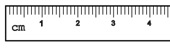
\includegraphics[width=0.5\textwidth]{ruler.jpg}
		
		\begin{solution}
			Half the smallest division, so 0.05 cm
		\end{solution}
		
		\item protractor
		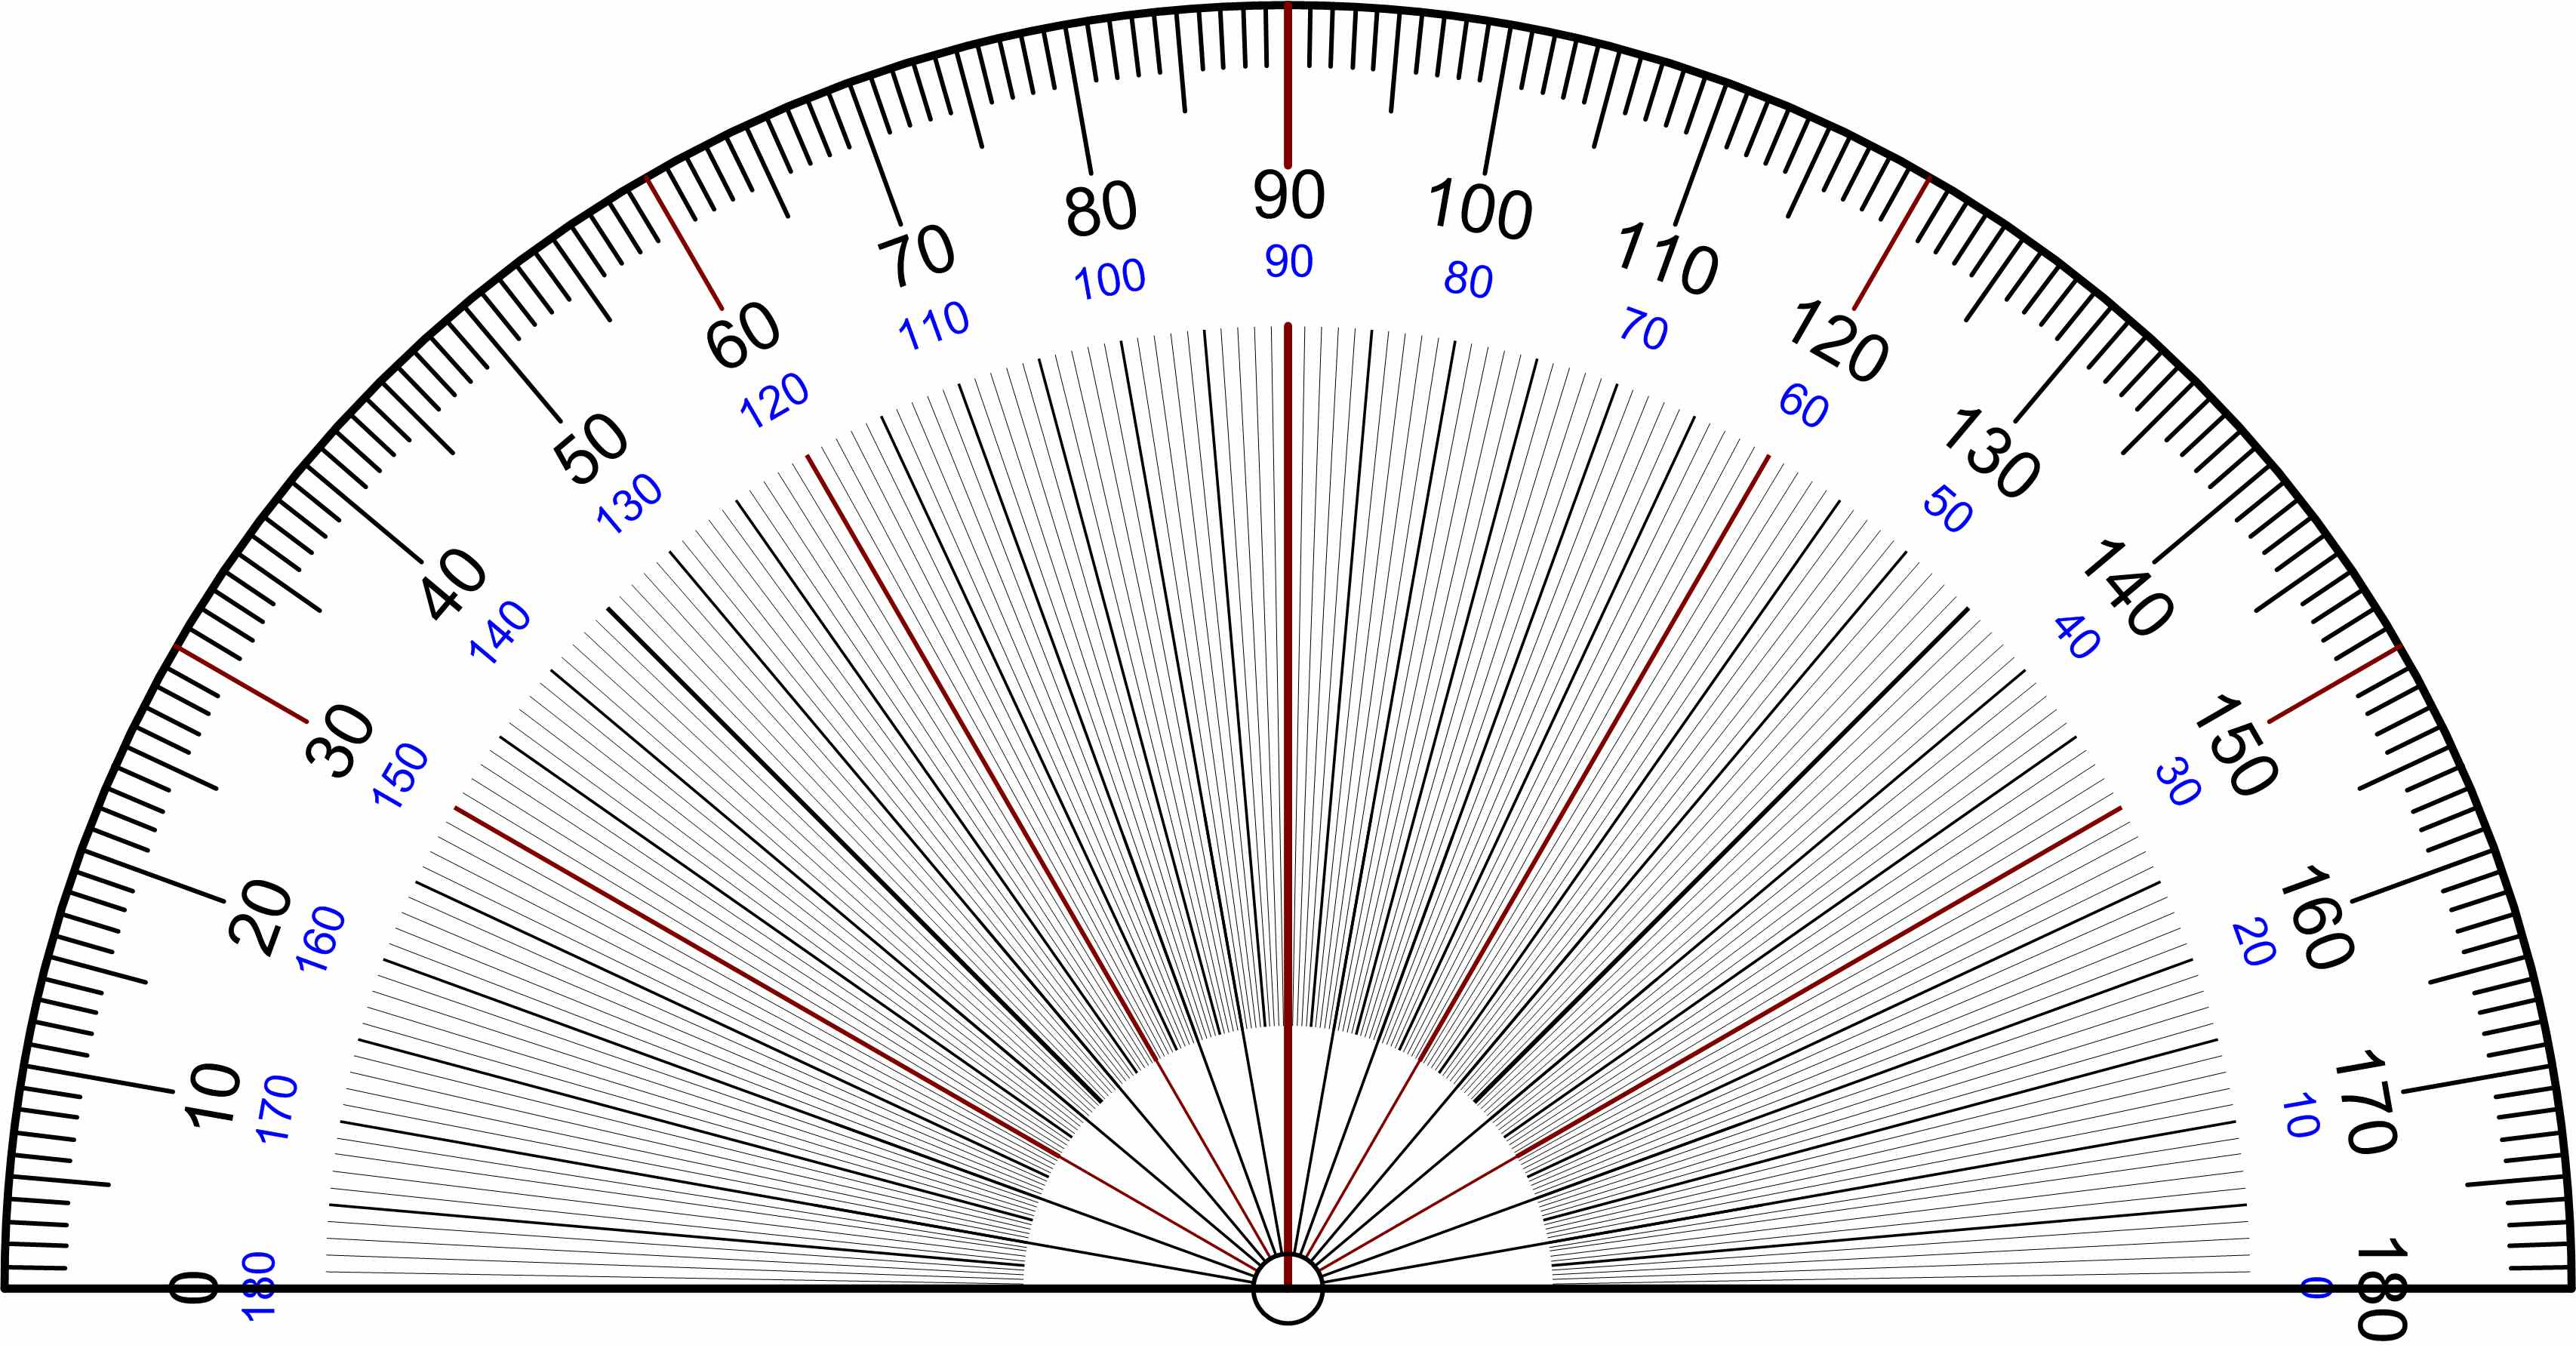
\includegraphics[width=0.8\textwidth]{Protractor_Rapporteur_Degrees_V3.jpg}
		
		\begin{solution}
			Half the smallest division, so 0.5 degrees
		\end{solution}
		
		\item watch
		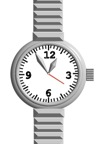
\includegraphics[width=0.3\textwidth]{watch.jpg}
		
		\begin{solution}
			Half the smallest division, so 0.5 seconds
		\end{solution}
	\end{enumerate}
	
	\item Measure the length of the pencil using the ruler next to it. Estimate the \textbf{relative} uncertainty in the measurement.
	
	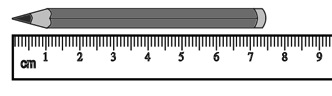
\includegraphics[width=\textwidth]{pencil-ruler.jpg}
	
	\begin{solution}
		Will accept 7.4 to 7.6 cm for estimated length. Relative uncertainty is given by
		\begin{align*}
		\textrm{relative uncertainty} &= \frac{\Delta a}{a} \\
		 &= \frac{0.05\:\mathrm{cm}}{7.5\:\mathrm{cm}} \\
		 &= 0.0067 \\
		 &= 0.67\%
		\end{align*}
	\end{solution}
	
	\item Using the instruments from Problem~\ref{fm1:qu:instrument}, you take the following measurements for the distance a toy car travels in 10 seconds during each of 5 trials: 157 cm, 175 cm, 162 cm, 168 cm, 187 cm.
	\begin{enumerate}
		\item For the distance measurement, which is greater, the instrumental uncertainty of one of the measurements, or the random uncertainty associated with the set of measurements? Estimate the random uncertainty.
		
		\begin{solution}
			Random uncertainty is given by standard deviation of the set of trials. Using spreadsheet program LibreOffice and its formula for standard deviation, STDEV, I get random uncertainty of 11.7 cm. Instrumental uncertainty is only 0.05 cm, so random is much larger.
		\end{solution}
		
		\item Using the random uncertainty of the distance measurement and the instrumental uncertainty of the time measurement, what are the relative uncertainties of the distance and time measurements, respectively?
		
		\begin{solution}
			For distance, relative uncertainty is
			\begin{align*}
				\frac{\Delta a}{a} &= \frac{11.7\:\mathrm{cm}}{169.8\:\mathrm{cm}} \\
				&= 6.89\%
			\end{align*}
			
			where I calculated the average value for the distance, 169.8 cm. For time,
			
			\begin{align*}
			 \frac{\Delta a}{a} &= \frac{0.5\:\mathrm{s}}{10\:\mathrm{s}} \\
			 &= 5\%
			\end{align*}
		\end{solution}
		
		\item Which measurement is the most uncertain, distance or time?
		
		\begin{solution}
			Distance, since the relative uncertainty is greater than for time.
		\end{solution}
	\end{enumerate}
	
	\item Using the average distance above, calculate the average speed of the toy car. Use the formula for propagation of uncertainty from the lab manual appendix to determine the uncertainty in the speed.
	
	\begin{solution}
		I calculate the speed using the kinematic equation,
		
		\begin{align*}
		 x = v t \,.
		\end{align*}
		
		Solving for $v$,
		
		\begin{align*}
		 v &= \frac{x}{t} \\
		 &= \frac{169.8\:\mathrm{cm}}{10\:\mathrm{s}} \\
		 &= 16.98\:\mathrm{cm}/\mathrm{s}
		\end{align*}
		
		This is a division of two quantities, so I use the corresponding formula to propagate error:
		
		\begin{align*}
		 \Delta{v}/v &= \sqrt{\left(\Delta x / x \right)^2 + \left(\Delta t / t \right)^2} \\
		 &= \sqrt{\left(0.0689 \right)^2 + \left(0.05 \right)^2} \\
		 &= 0.0851
		\end{align*}
		
		Solving for $\Delta v$ and substituting $v$ from above,
		
		\begin{align*}
		 \Delta v &= 0.0851 v \\
		 &= 0.0851 \times 16.98\:\mathrm{cm}/\mathrm{s} \\
		 &= 1.445\:\mathrm{cm}/\mathrm{s}
		\end{align*}
	\end{solution}
	
\end{enumerate}

\end{document}